
\begin{figure}
\centering
\begin{subfigure}{.5\textwidth}
  \centering
  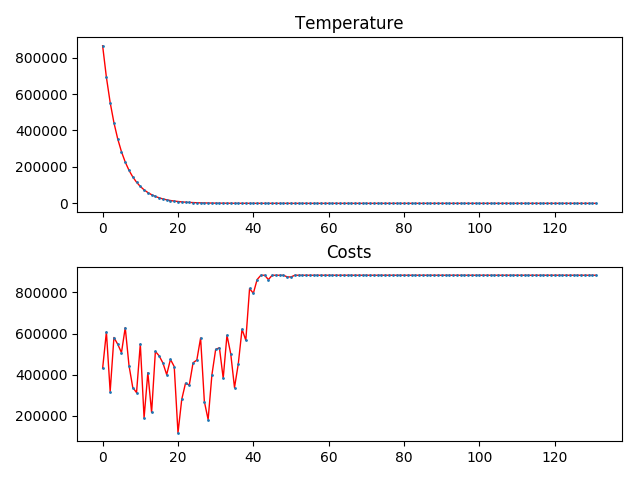
\includegraphics[width=1\linewidth]{results/cut12/3/plot}
  \label{fig:sub1}
\end{subfigure}%
\begin{subfigure}{.5\textwidth}
  \centering
  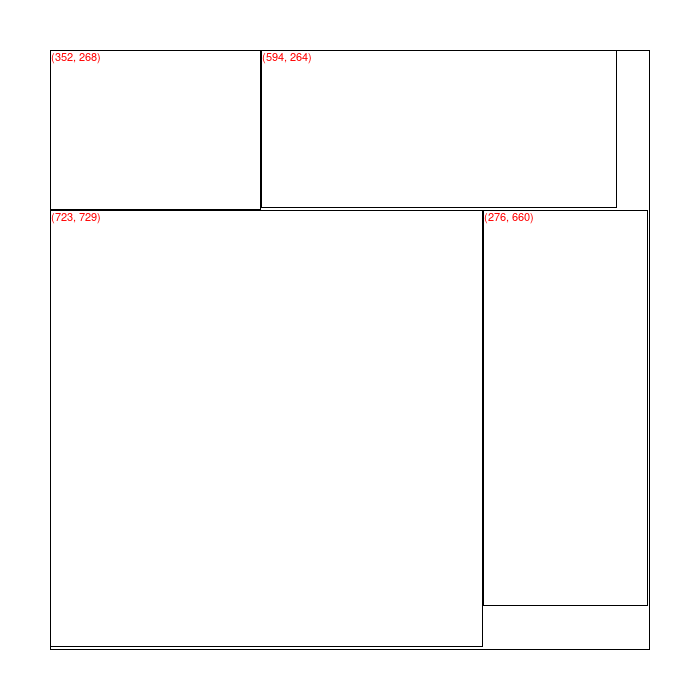
\includegraphics[width=1\linewidth]{results/cut12/3/cut}
  \label{fig:sub2}
\end{subfigure}
\caption{Instancia cut12.txt, Solução: 975059, desperdício de 2.49\% de 1000x1000, {(599, 269): 1, (359, 728): 1, (352, 268): 1, (640, 716): 1}}
\label{fig:test}
\end{figure}


\begin{figure}
\centering
\begin{subfigure}{.5\textwidth}
  \centering
  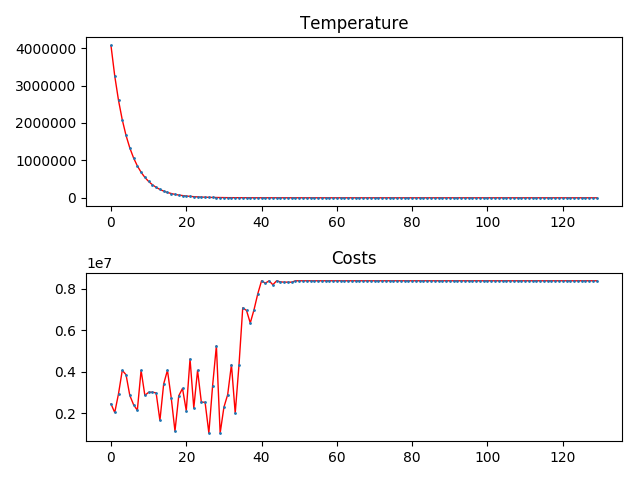
\includegraphics[width=1\linewidth]{results/cut13/1/plot}
  \label{fig:sub1}
\end{subfigure}%
\begin{subfigure}{.5\textwidth}
  \centering
  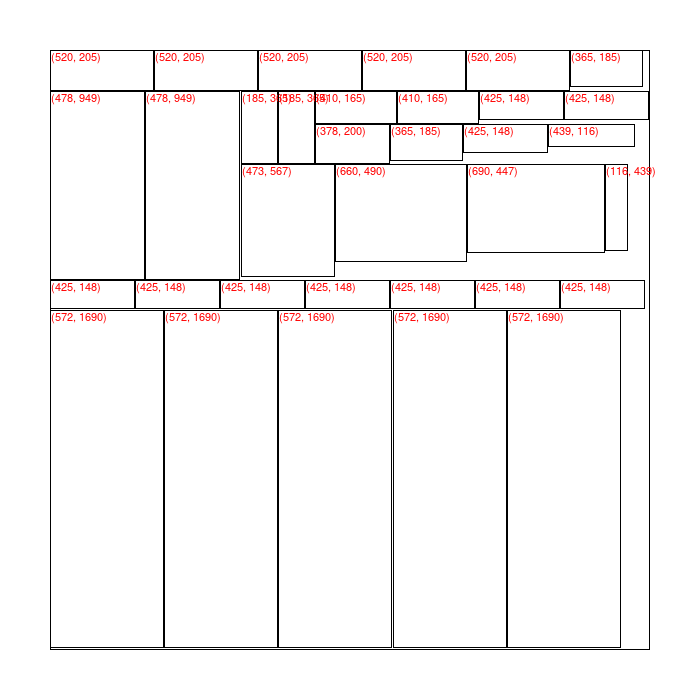
\includegraphics[width=1\linewidth]{results/cut13/1/cut}
  \label{fig:sub2}
\end{subfigure}
\caption{Instancia cut13.txt, Solução: 8212359, desperdício de 8.75\% de 3000x3000, {(540, 530): 1, (496, 555): 1, (520, 205): 1, (365, 185): 1, (116, 439): 1, (949, 445): 2, (296, 425): 1, (572, 1890): 5, (410, 165): 2, (148, 425): 1, (530, 540): 1, (205, 520): 1, (200, 378): 1, (567, 473): 1}}
\label{fig:test}
\end{figure}

